% !Mode:: "TeX:UTF-8" 

\BiChapter{基于注意力机制的卷积神经网络社交媒体文本立场分析}{Methods of inserting figures}

\BiSection{引言}{Figures inserting standard from graduate school}
近年来,深度学习的研究越来越深入,在各个领域也都获得了不少突破性的进展。基于注意力(attention)机制的神经网络成为了最近神经网络研究的一个热点,引起了研究者的广泛关注。在神经网络实现预测任务时,引入注意力机制能使训练重点集中在输入数据的相关部分,而不是无关部分。在社交媒体文本立场分析任务中, 不管是基于传统特征工程的机器学习模型SVM和基于端到端的深度学习的RNNs,CNNs等神经网络模型,都忽略主题目标信息对社交媒体立场分析的重要作用,这样建立模型存在的不合理性,为了更好的引入主题目标信息帮助提高社交媒体文本立场分析任务的性能,在本章引入基于注意力机制的神经网络模型。通过不同的权重,注意力机制能根据主题目标更好的对微博或者文本信息进行不同重要性的关注,使模型更加聚焦在对主题目标立场分析重要的信息上。实验结果表明,基于注意力机制的神经网络模型在社交媒体文本立场分析任务中取得了相当不错的效果,证明了注意力机制的有效性。

本章 4.2 节首先介绍深层记忆网络的重要机制及架构, 4.3 节介绍深层记忆网络在社交媒体文本立场分析中的应用,4.4 节介绍实验设置和结果的分析,4.5 节作出本章小结。

\BiSection{注意力机制的卷积神经网络模型的社交媒体文本立场分析}{Captions and descriptions of figures}

近年来,基于深度学习已经在图像识别、语音识别和自然语音处理上上获得了重要的进展。在自然语言处理任务中,注意力机制在神经网络机器翻译、序列标注、层次性文本分类上取得突破性提高。注意力机制将对信息呈现不同的关注程度,通过聚焦在重要的信息上,达到模型性能的特点。本节!!!!!!
\BiSubsection{注意力机制}{}
注意力机制最早应用在图像识别领域上,研究人员研究的动机其实也是受到人类注意力机制的启发。人们在进行观察图像的时候,并不是一次就把整幅图像的每个位置像素都看过,大多是根据需求将注意力集中到图像的特定部分。而且人类会根据之前观察的图像学习到未来要观察图像注意力应该集中的位置。

注意力机制除在图像识别和语音识别上取得巨大的成功,近期在基于RNNs的端到端的编码解码的机器翻译、序列标注和层次文本分类等任务取得突破。在自然语言处理任务中,首先引入注意力机制的是神经网络机器翻译。神经网络机器翻译其实就是一个典型的序列到序列模型,也就是一个编码解码模型。由于基于注意力机制的卷积神经网络模型的注意力机制很类似于机器翻译中的注意力机制,这里将简单介绍下机器翻译中的编码解码注意力机制模型。
\begin{figure}[htbp]
	\centering
	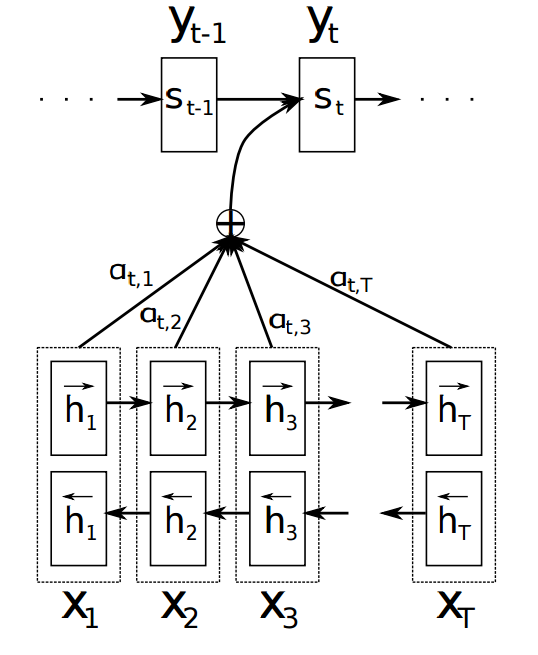
\includegraphics[width = 0.6\textwidth]{NMT.png}
	\caption[rnn_vanish]{注意力机制神经翻译模型}
\end{figure}

传统的神经翻译模型编码阶段里面用的是RNNs模型,这样每个单词的表达不仅能包含前一个单词的信息,还可以包含后一个; RNNs按输入序列的顺序,生成同样顺序的隐藏层状态,这样它就既包含当前单词的前一个单词信息,也包含后一个信息; 这个状态之后将被用于解码阶段部分。
\begin{equation}\label{lstm_f} h_t = f(x_t,h_{t-1}) \end{equation}

其中编码信息为
\begin{equation}\label{lstm_f} c = q(\lbrace h_1,...h_{T_x} \rbrace ) \end{equation}

其中$h_t$是时间$t$的隐藏状态,$c$向量是从序列信息得到的压缩向量,通常$f$和$q$是非线性函数,例如SutSkever[XXX]等用的是LSTM作为$f$函数,把前向循环网络的最后一个隐状态当做最好的压缩向量,$q(\lbrace h_1,...h_{Tx} \rbrace )=h_T$

在解码阶段,解码器的作用是根据编码的信息和已经输出的信息来预测下一个词最有可能的单词,可以用下面公式~\ref{rnndecoder}~表示
\begin{equation}\label{rnndecoder} p(y) = \prod_{t=1}^{T} p(y_t|\lbrace y1,...,y_{t-1} \rbrace , c) \end{equation}
当$y=(y1,...,y_{T})$,若用RNN式的结构,每个的条件概率如公式\ref{rnndecodery}
\begin{equation}\label{rnndecodery} p(y_t|\lbrace y1,...,y_{t-1} \rbrace , c) = g(y_{t-1},s_t, c)\end{equation}

而基于注意力机制的神经翻译模型的条件概率公式如下
\begin{equation}\label{} p(y_t|\lbrace y1,...,y_{t-1},x \rbrace , c) = g(y_{t-1},s_t, c_i)\end{equation}
其中$s_i$是RNN的隐状态,其中的计算公式如下
\begin{equation}\label{} s_i = f(s_{i-1},y_{i-1}, c_i)\end{equation}
其中从传统的神经翻译模型做出的改进是对于每一个不同的输出,它所依据的上下文压缩向量$c_i$不在是同一个压缩向量$c$,$c_i$的计算是通过$(h_1,...,h_{T_x})$的加权所得。$h_i$虽然包含所以所有的输入信息,但是主要存储了$x_i$的信息。其中$c_i$的计算公式如\ref{c1}所示
\begin{equation}\label{c1} c_i = \sum_{j=1}^{T_x} \alpha_{ij}h_i\end{equation}
其中注意力变量$\alpha{ij}$的计算公式如下
\begin{equation}\label{alpha} \alpha_{ij} = \frac{exp(e_{ij})}{\sum_{k=1}^{T_x}exp(e_{ik})}\end{equation}
其中$e_{ij}$的计算公式如下
\begin{equation}\label{eij} \alpha_{ij} = a(s_{i-1},h_j)\end{equation}

注意力机制的加入使得神经网络翻译模型具有更强的对句子翻译建模能力,使模型在翻译当前词语时关注和词语的更相关的内容,忽略不相关的内容。通过可视化注意力$\alpha{ij}$可显示看出在翻译不同词语时,对原语言关注的内容是不一样的,例如在中文翻译中的注意力矩阵如下图\ref{english2china}所示
\begin{figure}[htbp]
	\centering
	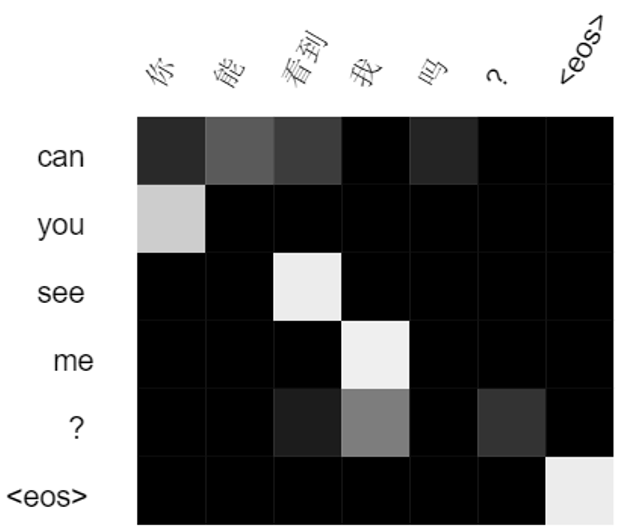
\includegraphics[width = 0.5\textwidth]{mnt_visual.jpg}
	\caption[english2china1]{中英文翻译注意力矩阵}
	\label{english2china}
\end{figure}

\BiSubsection{卷积神经网络}{xxl}

卷积原是常用在积分变换等领域的数学概念。现在被广泛应用于计算机视觉、自然语言处理和语音识别等任务中。卷积神经网络是对神经网络模型的改进。卷积层把原来的全连接改成局部连接权值共享,既可以大大缩减参数个数,又可以适应不同区域统计特性一样的特征。下采样层可以利用局部信息采样特征图得到更低纬度的特征,提高模型的泛化能力,防止训练的分类器过拟合。

根据不同任务,卷积神经网络的输入矩阵处理方式也不全相同。用于图片分类时,输入矩阵为像素点矩阵,用于文本分类时,输入矩阵为相同维度的词向量以一行一个词拼接。卷积神经网络使用预设石村的卷积核作为过滤器,与输入矩阵做卷积操作。

以文本卷积神经网络为例,当输入矩阵的词向量维数为$d$,句子长度为$l$,输入矩阵的大小为$A\in R^{l\times d}$, $A[i:j]$表示输入矩阵中从第$i$行到第$j$行的子矩阵。尺寸为$h$的过滤器对矩阵$A$做卷积操作,输出矩阵$O\in R^{s-h+1}$如公式~\ref{conv1}~所示,
\begin{equation}\label{conv1}
O_i=W\cdot A[i:i+h-1]
\end{equation}
其中,$i$为从1到$s-h+1$的数列。

将输出矩阵与偏置$b$相加,放入激活函数中处理,即可得到卷积层的输出$C_i$。

卷积层一般会连接下采样层。在自然语言处理任务重,下采样层通常使用KMAX池化函数,所以下采样层也被称为池化层。池化层既可以对卷积层的输出再次降维从而组合更大窗口范围的特征,同时也可以将不同尺寸的卷积核得到的特征构建为固定长度的输出,避免了不同输入矩阵大小表示的差异。之后的向量通常会连接Dropout层,随机抛弃一些节点,也是为了减少过拟合现象同时可以增强网络的训练效果。最后的全连接分类层通常使用softmax函数,基于多卷积核文本的CNN分类框架图如~\ref{multiCNN}~所示

\begin{figure}[htbp]
	\centering
	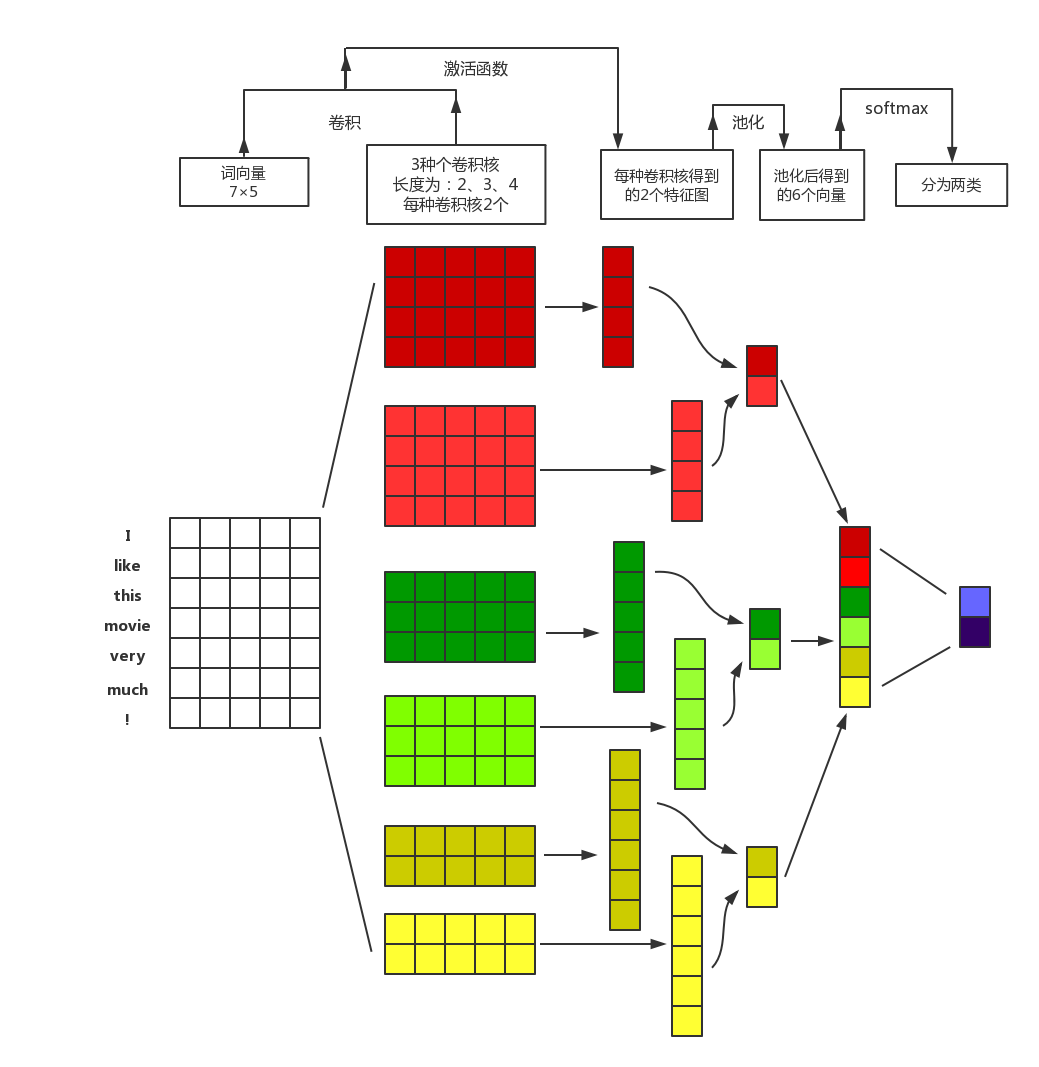
\includegraphics[width = 0.95\textwidth]{text_cnn.png}
	\caption{多卷积核文本CNN}
	\label{multiCNN}
\end{figure}

\BiSubsection{注意力机制卷积神经网络社交媒体文本立场分析}{}
基于注意力机制在神经网络翻译模型、序列标注、层次文本分类等领域取得的成功。文本多卷积核CNN模型在文本分类上的也取得了较好的效果。在社交媒体的文本立场分析上,由于当前研究没有一种有效把主题目标信息以合适的方式结合在文本的立场分析中,但是主题目标对文本立场分析又有着举足轻重的影响。为了主题目标信息没有合适引入的缺点,本文提出一种以注意力机制引入主题目标信息,在注意力的基础上,用多卷积核文本CNN模型提取文本立场的模型,本节结合立场分析数据集中的中文实例数据,描述注意力机制卷积神经网络在该问题中的主要工作流程和重要计算方法。
\begin{figure}[htbp]
	\centering
	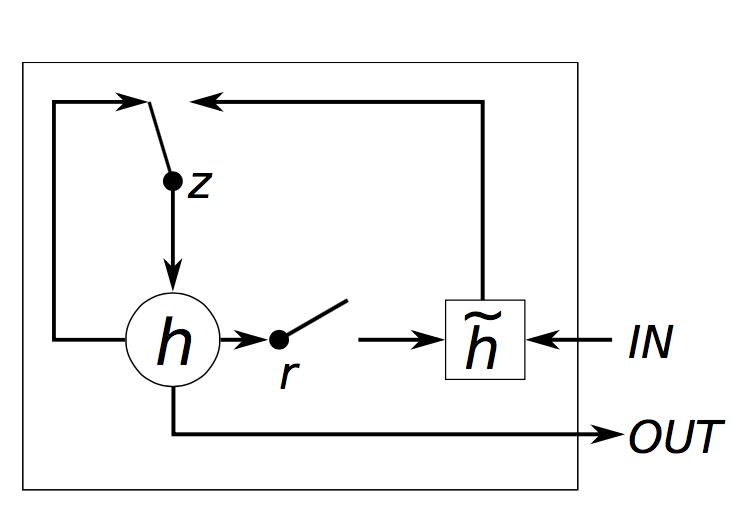
\includegraphics[width = 0.7\textwidth]{gru.png}
	\caption[rnn_vanish]{GRU内部结构}
	\label{gru}
\end{figure}
文本引入了双向GRU(Gated recurrent unit)用来编码文本信息,相对于RNN单元,GRU也能够缓解递归神经网络的梯度消失的问题,相对于LSTM单元,GRU具有更少的参数和更快的运算速度,因此本文利用例如GRU编码信息。相对于LSTM单元有输入门、遗忘门和输出门的三个门单元,按图~\ref{gru}~所示,GRU采取了一种更加简洁的建模方式,只需要保持更新门和重置门,更新门表示隐藏单元有多少信息需要保留下来,重置门表示都是隐藏单元信息参与输入的更新,同时也删除了LSTM的记忆单元,具体的门的更新和输出更新公式如下

\begin{equation}\label{conv1} z_t=\alpha_g(W_zx_t+U_zh_{t-1}+b_z) \end{equation}
\begin{equation}\label{conv1} r_t=\alpha_g(W_rx_t+U_rh_{t-1}+b_r) \end{equation}
\begin{equation}\label{conv1} h_t=z_t\odot h_{t-1} + (1-z_t)\odot \alpha(W_hx_t+U_h(r_t\odot h_{t-1})+b_h) \end{equation}



本节以“深圳禁摩限电”为话题目标,微博文本“支持深圳交警。电单车继续治理”为例,按本节模型的5个层次,描述注意力机制卷积神经网络的立场分析的过程,具体模型的结构如图~\ref{GRU_CNN}~所示

\begin{figure}[htbp]
	\centering
	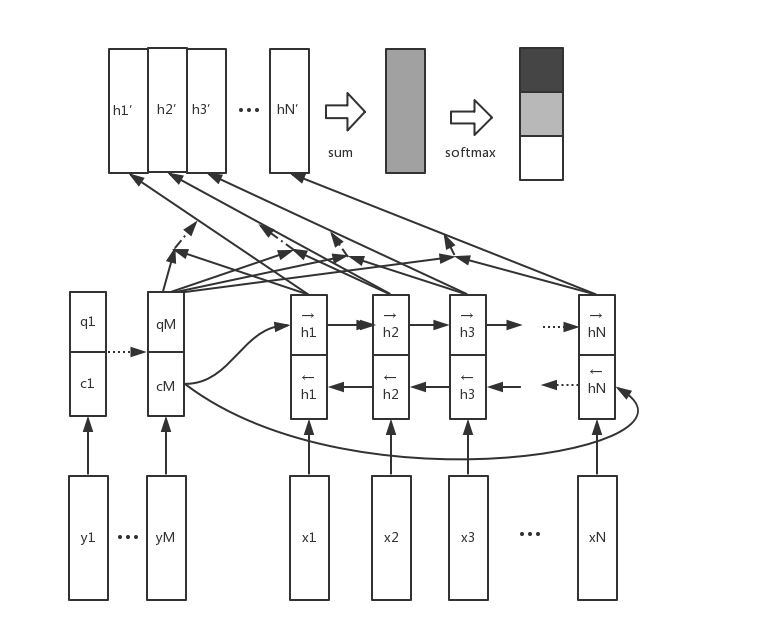
\includegraphics[width = 0.61\textwidth]{a_bi_gru_cnn.png}
	\caption[]{条件编码长短期记忆}
	\label{GRU_CNN}
\end{figure}

(1) 输入层

先将话题目标和微博文本经过预处理操作,然后通过分词工具把话题目标和微博文本进行划分,对于同一个话题目标,微博文本分词后句子长度有可能不一致,为了方便后续神经网络框架中的批量的并行计算,英文语料统计选择30为固定长度,中文语料统计后截取50为固定长度,长度超过固定长度进行截断操作,不够的进行补齐词表中规定 <PAD> 关键词。如上述微博文本最后转换成”支持深圳交警。电单车继续治理 <PAD> ... <PAD>“,而话题目标也需要进行分词操作,例如例子中“深圳禁摩限电”根据结巴分词分割成“深圳”、“禁摩”和“限电”三个词组。经过此层后主题目标信息和微博文本信息可以转换成以下形式,m,n分布为主题目标和微博文本的长度。
\begin{equation}\label{target_info} Target= \lbrace w_1,w_2...w_m\rbrace \end{equation}
\begin{equation}\label{text_info} Text=\lbrace w'_1,w'_2...w'_n\rbrace  \end{equation}

(2)词向量嵌入层

词向量的嵌入层,此层的功能是对输入的每一次词检索其词向量 (lookup操作),后续实验词向量的预训练由 GloVe 模型在大量无监督语料上训练可得,预训练的词向量维度为200,且把词向量设置为可训练,随神经网络模型的训练动态调整权重。经过此层后主题目标信息和微博文本信息可以转换成以下形式。
\begin{equation}\label{target_info} Target_v= \lbrace y_1,y_2...y_m\rbrace \end{equation}
\begin{equation}\label{text_info} Text_v=\lbrace x_1,x_2...x_n\rbrace \end{equation}

(3)主题目标编码与文本编码层

由于微博和Twitter文本立场分析中的主题目标包含的词语相对较少,为了减少模型的参数空间,因此编码主题目标信息的方法是平均所有词向量。微博或Twiiter文本包含了文本立场分析的绝大部分信息,双向的GRU单元能比单向更好抽取文本中的信息,对于当前词的隐藏状态包含前向和后向的GRU隐状态。具体的转换如公式所示。
\begin{equation}\label{target_info} q=\frac{\sum_{m}^{i=1}y_i}{m} \end{equation}
\begin{equation}\label{target_info} h^→_i = GRU^→(h^→_{i-1}, x_i) \end{equation}
\begin{equation}\label{text_info}  h^←_i = GRU^→(h^←_{i+1}, x_i) \end{equation}
\begin{equation}\label{text_info}  h_i = [h^→_{i-1}, h^←_{i+1}] \end{equation}

(4)注意力机制计算与基于注意力的隐藏状态合成

通过结合主题目标编码信息$q$和微博的文本信息的基于双向GRU模型的隐状态$h_i$,分布计算主题目标对每个词的关注程度,对于文本分析影响大的词,注意力机制会给予大的权重,反过来对于无用信息,注意力机制则会给予小的权重。分别计算每个词的权重后,原隐状态点城注意力的权重形成基于注意力的隐藏状态,具体的计算公式如下
\begin{equation}\label{conv1} e_i=att(h_i,q)=W^t_n(tanh(W_{ah}h_i+W_{aq}q+b_a))+b_m \end{equation}
\begin{equation}\label{conv1} a_i=\frac{exp(e_i)}{\sum_{N}^{n=1}exp(e_n)} \end{equation}
\begin{equation}\label{conv1} h'_i=a_i \odot h_i \end{equation}

(5)多窗口核卷积与池化操作

模型初始化不同大小的过滤器窗口,每种尺寸的窗口随机初始化若干参数。图中所示窗口大小w为2,并随机初始化多个不同的过滤器。所得向量将送入修正线性单元(Rectified Linear Units,ReLU)等非线性目标激活函数中,池化操作将卷积层中每个卷积过滤器所得长度为N-h+1的向量使用最大池化操作(max pooling),池化操作能减低参数维度,减少计算复杂度。具体公式如下
\begin{equation}\label{conv1} c_i=W*h[i:i+w-1]+b \end{equation}
\begin{equation}\label{conv1} c=Max(c_1,c_2,...,c_n) \end{equation}

(6)全连接分类层
把每个卷积核经过池化操作的值拼接在一起作为模型最后的特征向量,对特征向量连接一个以三个输出单元的全连接层。全连接层输出外接Softmax归一化函数,输出的值为归一化到0-1之间的实数值,代表的意义为模型分类到某一个立场的概率,具体公式如下。
\begin{equation}\label{conv1} ouput_i=Softmax(W_{h3}C+b_{h3}) \end{equation}


R$R~Max$


\begin{equation}\label{conv1} z_t=\alpha_g(W_zx_t+U_zh_{t-1}+b_z) \end{equation}
\begin{figure}[htbp]
	\centering
	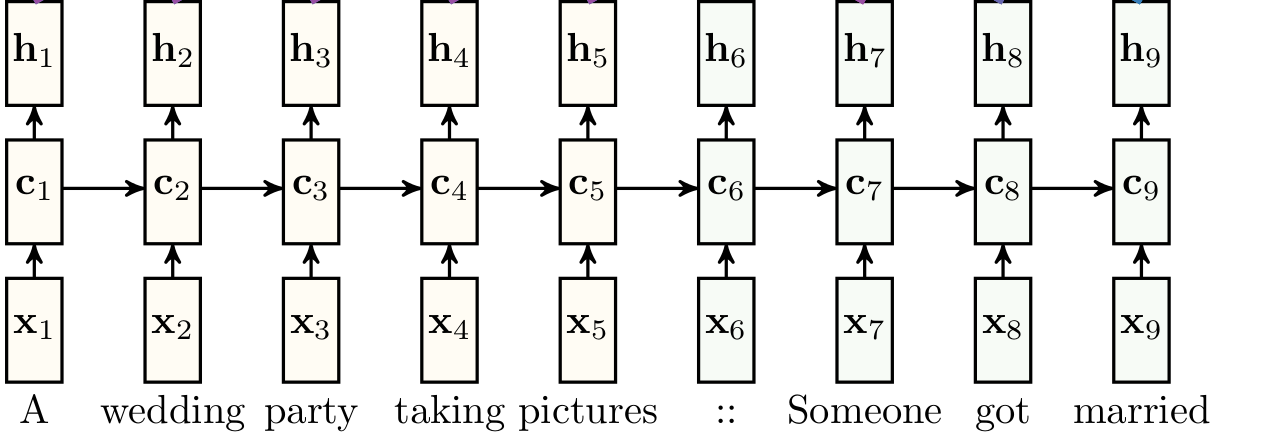
\includegraphics[width = 0.8\textwidth]{conditional_encoding.png}
	\caption[rnn_vanish]{条件编码长短期记忆}
	\label{hehehe}
\end{figure}

